\phantomsection
\section*{Chapitre 4 : Construction du mod\`ele pr\'edictif et d\'etection d'anomalies}
\addcontentsline{toc}{section}{Chapitre 4 : Construction du mod\`ele pr\'edictif et d\'etection d'anomalies}

\bigskip

Ce chapitre pr\'esente la mise en \oe{}uvre concr\`ete de la d\'emarche pr\'edictive.
Apr\`es avoir d\'ecrit le jeu de donn\'ees et les variables retenues, nous comparons
plusieurs mod\`eles, exposons les m\'etriques utilis\'ees pour les \'evaluer, puis
pr\'esentons les mod\`eles s\'electionn\'es et les pr\'evisions obtenues pour
l'exercice 2025. Une derni\`ere section traite de la d\'etection d'anomalies
appliqu\'ee \`a ces pr\'evisions. Le chapitre se conclut par une synth\`ese et une
discussion honn\^ete des limites du travail.

%================================================================
\phantomsection
\subsection*{4.1 \quad Pr\'esentation et construction des donn\'ees}
\addcontentsline{toc}{subsection}{4.1 Pr\'esentation et construction des donn\'ees}
%================================================================

Cette section d\'ecrit l'origine du jeu de donn\'ees, la d\'emarche suivie pour
reconstituer les taux d'ex\'ecution au niveau de la ligne budg\'etaire \`a partir
des sources publiques disponibles, et les principales caract\'eristiques
statistiques de l'\'echantillon obtenu.

%----------------------------------------------------------------
\phantomsection
\subsubsection*{4.1.1 \quad Source et p\'erim\`etre des donn\'ees}
\addcontentsline{toc}{subsubsection}{4.1.1 Source et p\'erim\`etre des donn\'ees}
%----------------------------------------------------------------

Le jeu de donn\'ees est constitu\'e \`a partir de deux sources publiques compl\'ementaires.
D'une part, les \textbf{morasses budg\'etaires annuelles} publi\'ees avec les projets
de loi de finances (2020--2025), qui fournissent la nomenclature compl\`ete des lignes
budg\'etaires du Minist\`ere de la Justice ainsi que les cr\'edits initiaux par ligne.
D'autre part, les \textbf{rapports d'ex\'ecution trimestriels} de la Tr\'esorerie
G\'en\'erale du Royaume (TGR), qui renseignent les taux d'ex\'ecution agr\'eg\'es par
cat\'egorie de d\'epense.

Le tableau~\ref{tab:volumetrie} r\'esume la volum\'etrie du jeu de donn\'ees final.

\begin{table}[H]
\centering\small
\caption{Volum\'etrie du jeu de donn\'ees.}
\label{tab:volumetrie}
\begin{tabular}{@{}lr@{}}
\toprule
\textbf{Dimension} & \textbf{Valeur} \\
\midrule
P\'eriode couverte                           & 2020--2025 (6 exercices) \\
Nombre de lignes budg\'etaires distinctes    & 130 \\
Nombre de programmes                         & 4 (P300--P303) \\
Nombre de r\'egions                          & 13 \\
Cat\'egories de d\'epense                    & 3 (Investissement, Mat\'eriel, Personnel) \\
Trimestres par ligne et par ann\'ee          & 4 (T1--T4) \\
Nombre total d'observations                  & 3\,120 \\
\bottomrule
\end{tabular}
\end{table}

%----------------------------------------------------------------
\phantomsection
\subsubsection*{4.1.2 \quad Construction du jeu de donn\'ees}
\addcontentsline{toc}{subsubsection}{4.1.2 Construction du jeu de donn\'ees}
%----------------------------------------------------------------

La TGR publie les taux d'ex\'ecution agr\'eg\'es par cat\'egorie de d\'epense, mais
pas par ligne budg\'etaire individuelle. La morasse, de son c\^ot\'e, fournit la
liste exhaustive des lignes et leur cr\'edit initial. L'objectif a \'et\'e de
\textbf{combiner ces deux sources} pour reconstituer un jeu de donn\'ees aussi
proche que possible de la r\'ealit\'e ministerielle. La proc\'edure tient en
trois id\'ees simples~:

\begin{enumerate}
    \item \textbf{On part des chiffres r\'eels.} Les taux trimestriels par cat\'egorie
    publi\'es par la TGR (2020--2025) constituent l'ancrage quantitatif du jeu de
    donn\'ees. Aucune valeur n'est invent\'ee~: ces taux sont des chiffres officiels.

    \item \textbf{On r\'epartit ces taux sur les vraies lignes budg\'etaires.} La
    nomenclature programme\,$\rightarrow$\,projet\,$\rightarrow$\,r\'egion\,$\rightarrow$\,ligne
    est extraite directement des morasses. Chaque ligne re\c{c}oit un profil
    d'ex\'ecution coh\'erent avec sa nature (les travaux ex\'ecutent tard, les
    fournitures r\'eguli\`erement, le personnel lin\'eairement).

    \item \textbf{On v\'erifie que tout colle.} Apr\`es r\'epartition, la moyenne
    pond\'er\'ee des taux par ligne reproduit exactement les agr\'egats TGR. Si ce
    n'est pas le cas, les valeurs sont recal\'ees proportionnellement. Cette
    contrainte garantit qu'aucune statistique officielle n'est trahie.
\end{enumerate}

Le r\'esultat est un jeu de donn\'ees \textbf{r\'ealiste par construction}~: les
agr\'egats sont r\'eels, la structure analytique est r\'eelle, seule la
distribution fine entre lignes d'un m\^eme programme est reconstitu\'ee selon
des hypoth\`eses op\'erationnelles plausibles.

%----------------------------------------------------------------
\phantomsection
\subsubsection*{4.1.3 \quad Statistiques descriptives}
\addcontentsline{toc}{subsubsection}{4.1.3 Statistiques descriptives}
%----------------------------------------------------------------

Avant de pr\'esenter les mod\`eles, il importe de caract\'eriser la dynamique des
taux d'ex\'ecution. Trois constats structurent l'ensemble de la suite.

\textbf{Premier constat~: la saisonnalit\'e est tr\`es marqu\'ee.} Le tableau~\ref{tab:stats-trimestre}
montre la progression typique des taux du T1 au T4, toutes cat\'egories confondues.

\begin{table}[H]
\centering\small
\caption{Statistiques du taux d'ex\'ecution par trimestre (toutes cat\'egories, 2020--2025).}
\label{tab:stats-trimestre}
\begin{tabular}{@{}lcccc@{}}
\toprule
\textbf{Trimestre} & \textbf{Moyenne} & \textbf{\'Ecart-type} & \textbf{Min} & \textbf{Max} \\
\midrule
T1 &  6{,}7\,\% & 11{,}3\,\% &  0{,}0\,\% &  49{,}0\,\% \\
T2 & 24{,}5\,\% & 19{,}4\,\% &  1{,}2\,\% &  91{,}5\,\% \\
T3 & 49{,}6\,\% & 24{,}1\,\% &  8{,}6\,\% & 119{,}3\,\% \\
T4 & 90{,}6\,\% & 16{,}0\,\% & 49{,}1\,\% & 142{,}0\,\% \\
\bottomrule
\end{tabular}
\end{table}

\noindent
Seuls 25\,\% du budget en moyenne sont consomm\'es \`a la mi-ann\'ee (T2), contre 91\,\%
en fin d'exercice (T4). C'est pr\'ecis\'ement cet \'ecart qui rend la pr\'evision T4
non triviale et utile~: au 30~juin, l'essentiel de l'ex\'ecution reste \`a venir.

\textbf{Deuxi\`eme constat~: les cat\'egories ont des comportements radicalement
diff\'erents.} Le tableau~\ref{tab:stats-categorie} d\'etaille les statistiques du
taux T4 par cat\'egorie de d\'epense.

\begin{table}[H]
\centering\small
\caption{Statistiques du taux d'ex\'ecution T4 par cat\'egorie budg\'etaire.}
\label{tab:stats-categorie}
\begin{tabular}{@{}lccccc@{}}
\toprule
\textbf{Cat\'egorie} & \textbf{Nb obs.} & \textbf{Moyenne T4} & \textbf{\'Ecart-type} & \textbf{Min} & \textbf{Max} \\
\midrule
Investissement & 630 & 88{,}2\,\% & 15{,}8\,\% & 49{,}1\,\% & 135{,}6\,\% \\
Mat\'eriel     & 144 & 100{,}5\,\% & 13{,}0\,\% & 76{,}0\,\% & 142{,}0\,\% \\
Personnel      &   6 &  99{,}5\,\% &  1{,}5\,\% & 97{,}0\,\% & 101{,}5\,\% \\
\bottomrule
\end{tabular}
\end{table}

\noindent
Le \textbf{Personnel} affiche une variance quasi nulle ($\sigma = 1{,}5$\,points)~:
ces d\'epenses sont m\'ecaniques et parfaitement pr\'evisibles. Le \textbf{Mat\'eriel}
pr\'esente une variabilit\'e mod\'er\'ee. L'\textbf{Investissement}, en revanche,
montre la plus forte dispersion ($\sigma = 15{,}8$\,points) et des valeurs extr\^emes
allant de 49\,\% \`a 136\,\% : c'est la cat\'egorie la plus difficile \`a anticiper, et
celle pour laquelle un mod\`ele pr\'edictif apporte le plus de valeur.

\textbf{Troisi\`eme constat~: l'Investissement concentre les enjeux.} Les figures~\ref{fig:seasonality-inv} \`a~\ref{fig:seasonality-pers}
visualisent les profils saisonniers par cat\'egorie. L'investissement ex\'ecute moins
de 10\,\% en T1--T2 puis 70\,\% en T4~; c'est ce comportement tardif qui justifie
l'existence m\^eme d'un syst\`eme d'alerte pr\'ecoce.

\begin{figure}[H]
    \centering
    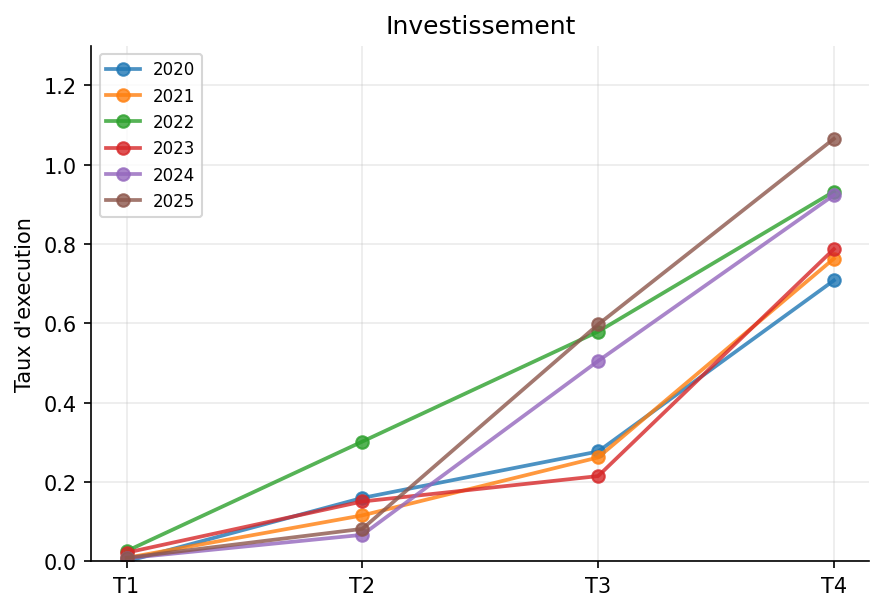
\includegraphics[width=0.55\textwidth]{figures/seasonality_investissement.png}
    \caption{Profil saisonnier du taux d'ex\'ecution --- D\'epenses d'Investissement (2020--2025).}
    \label{fig:seasonality-inv}
\end{figure}

\begin{figure}[H]
    \centering
    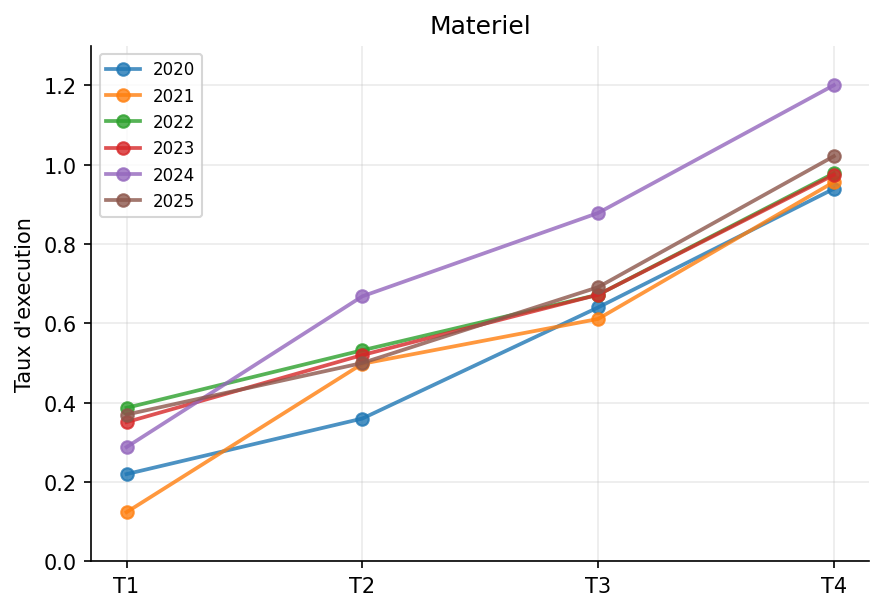
\includegraphics[width=0.55\textwidth]{figures/seasonality_materiel.png}
    \caption{Profil saisonnier du taux d'ex\'ecution --- D\'epenses de Mat\'eriel (2020--2025).}
    \label{fig:seasonality-mat}
\end{figure}

\begin{figure}[H]
    \centering
    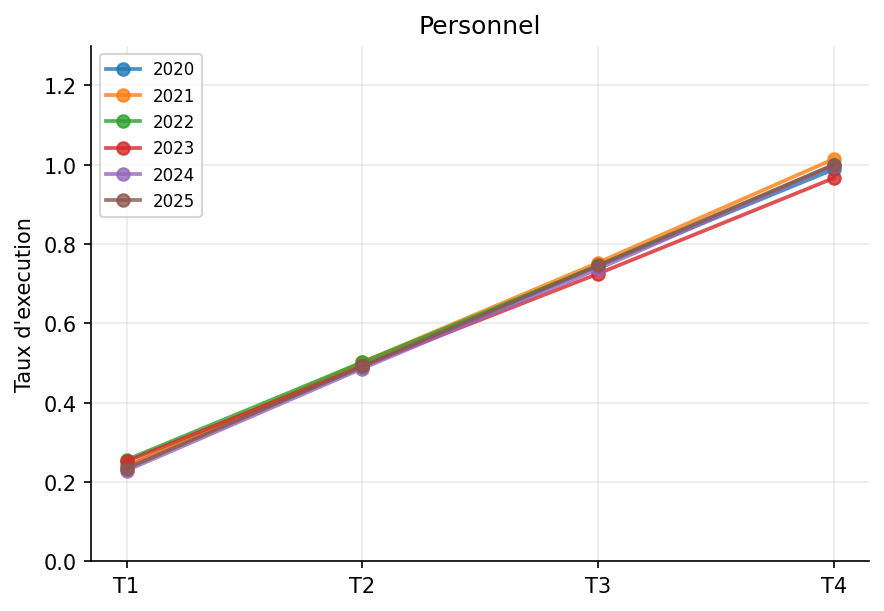
\includegraphics[width=0.55\textwidth]{figures/seasonality_personnel.png}
    \caption{Profil saisonnier du taux d'ex\'ecution --- D\'epenses de Personnel (2020--2025).}
    \label{fig:seasonality-pers}
\end{figure}

\noindent
Ces trois constats motivent directement les choix m\'ethodologiques qui suivent~:
des mod\`eles distincts par cat\'egorie (4.5), des variables explicatives privil\'egiant
l'historique r\'ecent (4.2), et une m\'ethode de d\'etection d'anomalies cibl\'ee sur
les sous-ex\'ecutions atypiques au T2 (4.6).

%================================================================
\phantomsection
\subsection*{4.2 \quad Variables utilis\'ees pour la pr\'ediction}
\addcontentsline{toc}{subsection}{4.2 Variables utilis\'ees pour la pr\'ediction}
%================================================================

Cette section pr\'esente la variable cible que les mod\`eles cherchent \`a pr\'edire,
les variables explicatives retenues, et l'encodage utilis\'e pour les variables
qualitatives.

%----------------------------------------------------------------
\phantomsection
\subsubsection*{4.2.1 \quad Variable cible (taux T4)}
\addcontentsline{toc}{subsubsection}{4.2.1 Variable cible (taux T4)}
%----------------------------------------------------------------

La variable cible est le \textbf{taux d'ex\'ecution annuel d'une ligne budg\'etaire},
mesur\'e en fin d'exercice (au 31~d\'ecembre)~:
$$
\text{taux T4} = \frac{\text{cr\'edits effectivement ex\'ecut\'es au cours de l'ann\'ee}}
                       {\text{cr\'edits inscrits en loi de finances}}
$$

\noindent
Une valeur de 1{,}00 signifie que la ligne a consomm\'e exactement son enveloppe annuelle~;
0{,}80 indique une sous-ex\'ecution de 20 points~; les valeurs sup\'erieures \`a 1
correspondent \`a des d\'epassements (rares, possibles en mati\`ere de Mat\'eriel et
de Personnel via les cr\'edits suppl\'ementaires). Le seuil m\'etier de 80\,\% retenu
par les \'equipes de la Division de la Pr\'evision et de la Programmation
financi\`ere (DPPF, rattach\'ee \`a la Direction du Budget) sert de fronti\`ere
entre une ex\'ecution acceptable et une ex\'ecution \`a risque.

%----------------------------------------------------------------
\phantomsection
\subsubsection*{4.2.2 \quad Variables explicatives et justification du choix}
\addcontentsline{toc}{subsubsection}{4.2.2 Variables explicatives et justification du choix}
%----------------------------------------------------------------

Les variables explicatives ont \'et\'e choisies selon trois crit\`eres~: (i)~elles
doivent \^etre \textbf{disponibles au 30~juin}, date \`a laquelle la pr\'evision est
produite~; (ii)~elles doivent \^etre \textbf{informatives} sur la dynamique d'ex\'ecution~;
(iii)~elles doivent \^etre \textbf{interpr\'etables} pour les utilisateurs m\'etiers.
Le tableau~\ref{tab:variables} r\'esume les variables retenues.

\begin{table}[H]
\centering\small
\caption{Variables retenues pour la pr\'evision du taux d'ex\'ecution T4.}
\label{tab:variables}
\begin{tabular}{@{}p{4.2cm}p{8cm}c@{}}
\toprule
\textbf{Variable} & \textbf{Ce qu'elle mesure} & \textbf{Dispo. 30~juin} \\
\midrule
\texttt{taux\_T2} & Taux d'ex\'ecution observ\'e \`a mi-parcours (fin juin de l'ann\'ee en cours). Une valeur faible signale un retard d\'ej\`a engag\'e. & Oui \\[3pt]
\texttt{taux\_T1} & Taux observ\'e \`a fin mars~; capture le d\'emarrage de l'exercice. & Oui \\[3pt]
\texttt{taux\_T4\_lag} & Taux T4 de l'an pass\'e~: signal le plus fort du comportement habituel de la ligne. & Oui \\[3pt]
\texttt{taux\_T2\_lag} & Taux T2 de l'an pass\'e~: permet de comparer le rythme actuel \`a celui de l'an pr\'ec\'edent. & Oui \\[3pt]
\texttt{hist\_avg\_T3} & Moyenne historique du taux T3 sur les ann\'ees pr\'ec\'edentes~: capture si une ligne \og rattrape \fg{} historiquement entre T2 et T3. & Oui \\[3pt]
\texttt{lf\_ratio}, \texttt{lf\_share} & Dotation relative de la ligne et part dans son programme~: d\'etectent les dotations atypiques. & Oui \\[3pt]
\texttt{type\_enc}, \texttt{prog\_enc}, \texttt{reg\_enc}, \texttt{budget\_enc} & Type de d\'epense, programme, r\'egion, cat\'egorie budg\'etaire (encod\'es). & Oui \\[3pt]
\texttt{taux\_T3} & (mod\`ele actualis\'e en septembre) Taux observ\'e \`a fin septembre. & Septembre \\
\bottomrule
\end{tabular}
\end{table}

\noindent
La variable \texttt{taux\_T4\_lag} est typiquement la plus informative~: si une
ligne a ex\'ecut\'e 75\,\% l'an dernier, la pr\'evision de cette ann\'ee gravite
naturellement autour de cette valeur. La variable \texttt{taux\_T2} apporte
l'information dynamique~: une ligne dont le taux T2 est anormalement faible
constitue un signal d'alerte ind\'ependamment de son historique.

%----------------------------------------------------------------
\phantomsection
\subsubsection*{4.2.3 \quad Encodage des variables cat\'egorielles}
\addcontentsline{toc}{subsubsection}{4.2.3 Encodage des variables cat\'egorielles}
%----------------------------------------------------------------

Les variables qualitatives (type de d\'epense, programme, r\'egion, cat\'egorie
budg\'etaire) sont encod\'ees en entiers via un mapping fixe~:

\begin{itemize}
    \item \textbf{Cat\'egorie budg\'etaire}~: \texttt{INVESTISSEMENT}~$\rightarrow$~0,
    \texttt{MATERIEL}~$\rightarrow$~1, \texttt{PERSONNEL}~$\rightarrow$~2.
    \item \textbf{Programme}~: P300~$\rightarrow$~0, P301~$\rightarrow$~1,
    P302~$\rightarrow$~2, P303~$\rightarrow$~3.
    \item \textbf{Type de d\'epense}~: \texttt{acquisitions}~$\rightarrow$~0,
    \texttt{equipements}~$\rightarrow$~1, \texttt{etudes}~$\rightarrow$~2,
    \texttt{fournitures}~$\rightarrow$~3, \texttt{travaux}~$\rightarrow$~4,
    \texttt{personnel}~$\rightarrow$~5.
    \item \textbf{R\'egion}~: encodage entier 0--12.
\end{itemize}

\noindent
Le \textit{label encoding} a \'et\'e pr\'ef\'er\'e au \textit{one-hot encoding}
pour deux raisons~: les mod\`eles \`a base d'arbres (XGBoost) g\`erent nativement
les variables ordinales sans souffrir de l'augmentation dimensionnelle~; et le
nombre limit\'e d'observations rend pr\'ef\'erable une repr\'esentation compacte.

%================================================================
\phantomsection
\subsection*{4.3 \quad Mod\`eles de pr\'ediction test\'es}
\addcontentsline{toc}{subsection}{4.3 Mod\`eles de pr\'ediction test\'es}
%================================================================

Quatre mod\`eles ont \'et\'e \'evalu\'es sur le m\^eme jeu de variables et le m\^eme
protocole de validation. Deux mod\`eles de r\'ef\'erence (na\"ifs) servent de
borne basse, et deux mod\`eles d'apprentissage automatique sont compar\'es.

%----------------------------------------------------------------
\phantomsection
\subsubsection*{4.3.1 \quad R\'ef\'erence na\"ive (moyenne historique, lag T4)}
\addcontentsline{toc}{subsubsection}{4.3.1 R\'ef\'erence na\"ive (moyenne historique, lag T4)}
%----------------------------------------------------------------

\textbf{Moyenne historique (\textit{Hist\_mean}).} Pour chaque ligne, on pr\'edit que
le taux T4 de l'ann\'ee cible sera \'egal \`a la moyenne des taux T4 observ\'es sur
les ann\'ees pass\'ees. C'est la borne basse \`a battre~: si un mod\`ele complexe ne
fait pas mieux que cette moyenne, son apport est nul.

\textbf{D\'ecalage annuel (\textit{Naive\_lag4}).} On pr\'edit simplement que le taux
T4 de l'ann\'ee cible sera \'egal \`a celui de l'ann\'ee pr\'ec\'edente. Ce mod\`ele
suppose une stabilit\'e temporelle parfaite et sert de second t\'emoin.

%----------------------------------------------------------------
\phantomsection
\subsubsection*{4.3.2 \quad Mod\`ele lin\'eaire r\'egularis\'e (Lasso)}
\addcontentsline{toc}{subsubsection}{4.3.2 Mod\`ele lin\'eaire r\'egularis\'e (Lasso)}
%----------------------------------------------------------------

Le mod\`ele Lasso effectue une r\'egression lin\'eaire avec une p\'enalisation $L_1$
sur les coefficients~:
$$
\min_{\boldsymbol\beta} \; \frac{1}{2N}\sum_{i=1}^{N}(y_i - \mathbf{x}_i^\top \boldsymbol\beta)^2
\;+\; \alpha \sum_j |\beta_j|
$$

\noindent
La p\'enalit\'e $L_1$ pousse certains coefficients exactement \`a z\'ero, r\'ealisant
une s\'election automatique de variables. Cela est particuli\`erement adapt\'e \`a
notre contexte~: l'\'echantillon est r\'eduit, et toutes les variables ne sont pas
\'egalement informatives selon la cat\'egorie. L'hyperparam\`etre $\alpha$ a \'et\'e
fix\'e \`a 0{,}01 apr\`es exploration. Les variables sont standardis\'ees en amont
via un \texttt{StandardScaler}.

%----------------------------------------------------------------
\phantomsection
\subsubsection*{4.3.3 \quad Mod\`ele \`a arbres boost\'es (XGBoost)}
\addcontentsline{toc}{subsubsection}{4.3.3 Mod\`ele \`a arbres boost\'es (XGBoost)}
%----------------------------------------------------------------

\textbf{XGBoost} (\textit{eXtreme Gradient Boosting}) construit s\'equentiellement un
ensemble d'arbres de d\'ecision peu profonds, chaque arbre corrigeant les erreurs
des pr\'ec\'edents. Cette architecture capture les non-lin\'earit\'es et les
interactions entre variables --- par exemple, l'effet conjoint d'une dotation
inhabituelle et d'un retard observ\'e en T2.

Les hyperparam\`etres retenus sont~:
\begin{center}
\texttt{n\_estimators=300}, \texttt{max\_depth=3},
\texttt{learning\_rate=0.05}, \texttt{subsample=0.8}, \texttt{reg\_alpha=0.1}.
\end{center}

\noindent
Une profondeur faible (\texttt{max\_depth=3}) et une r\'egularisation $L_1$ explicite
limitent le risque de surapprentissage sur un \'echantillon r\'eduit.

%================================================================
\phantomsection
\subsection*{4.4 \quad M\'etriques et protocole d'\'evaluation}
\addcontentsline{toc}{subsection}{4.4 M\'etriques et protocole d'\'evaluation}
%================================================================

L'\'evaluation poursuit un double objectif~: mesurer la qualit\'e absolue des
pr\'evisions et garantir que cette mesure refl\`ete les performances en conditions
r\'eelles, sans fuite d'information temporelle.

%----------------------------------------------------------------
\phantomsection
\subsubsection*{4.4.1 \quad RMSE et erreur moyenne}
\addcontentsline{toc}{subsubsection}{4.4.1 RMSE et erreur moyenne}
%----------------------------------------------------------------

Trois m\'etriques compl\'ementaires ont \'et\'e retenues~:

\begin{itemize}
    \item \textbf{RMSE} (\textit{Root Mean Squared Error})~:
    $\sqrt{\frac{1}{N}\sum_i (y_i - \hat y_i)^2}$.
    P\'enalise davantage les grosses erreurs.

    \item \textbf{MAE} (\textit{Mean Absolute Error})~:
    $\frac{1}{N}\sum_i |y_i - \hat y_i|$.
    \'Ecart absolu moyen, en points de taux.

    \item \textbf{MAPE} (\textit{Mean Absolute Percentage Error})~:
    $\frac{100}{N}\sum_i \left|\frac{y_i - \hat y_i}{y_i}\right|$.
    \'Ecart relatif moyen.
\end{itemize}

\noindent
Le RMSE constitue la m\'etrique principale~: une valeur de 0{,}08 signifie que le
mod\`ele se trompe en moyenne de 8 points de pourcentage sur le taux d'ex\'ecution
final, ce qui reste suffisant pour d\'eclencher une alerte budg\'etaire six mois
avant la cl\^oture.

%----------------------------------------------------------------
\phantomsection
\subsubsection*{4.4.2 \quad Validation crois\'ee walk-forward}
\addcontentsline{toc}{subsubsection}{4.4.2 Validation crois\'ee walk-forward}
%----------------------------------------------------------------

La validation crois\'ee classique (\textit{k-fold} al\'eatoire) m\'elange les ann\'ees
et cr\'ee une fuite temporelle~: le mod\`ele \og voit \fg{} l'avenir pendant
l'entra\^inement. Pour \'eviter ce biais, nous adoptons une validation
\textbf{walk-forward \`a fen\^etre expansive}~:

\begin{itemize}
    \item Pour pr\'evoir 2022, le mod\`ele est entra\^in\'e sur 2021 uniquement.
    \item Pour pr\'evoir 2023, sur 2021--2022.
    \item Pour pr\'evoir 2024, sur 2021--2023.
    \item Pour pr\'evoir 2025, sur 2021--2024.
\end{itemize}

\noindent
Ce protocole reproduit exactement la situation du gestionnaire~: pr\'edire une
ann\'ee \`a partir du seul historique pass\'e. Aucune information post\'erieure \`a
l'ann\'ee de pr\'evision n'intervient dans l'entra\^inement.

%----------------------------------------------------------------
\phantomsection
\subsubsection*{4.4.3 \quad \'Evaluation par cat\'egorie budg\'etaire}
\addcontentsline{toc}{subsubsection}{4.4.3 \'Evaluation par cat\'egorie budg\'etaire}
%----------------------------------------------------------------

Comme l'a montr\'e la section 4.1.3, les trois cat\'egories pr\'esentent des
comportements tr\`es diff\'erents. Une \'evaluation agr\'eg\'ee masquerait ces
disparit\'es~: un mod\`ele excellent sur Personnel mais m\'ediocre sur Investissement
afficherait un RMSE moyen acceptable, alors m\^eme que c'est sur l'Investissement
que les enjeux financiers sont les plus \'elev\'es. Toutes les m\'etriques sont
donc calcul\'ees \textbf{s\'epar\'ement par cat\'egorie} avant d'\^etre \'eventuellement
agr\'eg\'ees.

%================================================================
\phantomsection
\subsection*{4.5 \quad Mod\`eles retenus et r\'esultats}
\addcontentsline{toc}{subsection}{4.5 Mod\`eles retenus et r\'esultats}
%================================================================

Les r\'esultats r\'ev\`elent qu'aucun mod\`ele unique n'est optimal sur les trois
cat\'egories~; on retient donc une \textbf{architecture sp\'ecialis\'ee} qui combine
le meilleur mod\`ele pour chaque type de d\'epense.

%----------------------------------------------------------------
\phantomsection
\subsubsection*{4.5.1 \quad R\'esultats globaux par mod\`ele}
\addcontentsline{toc}{subsubsection}{4.5.1 R\'esultats globaux par mod\`ele}
%----------------------------------------------------------------

Le tableau~\ref{tab:global} pr\'esente les performances globales moyenn\'ees sur les
quatre folds de validation walk-forward et sur les trois cat\'egories.

\begin{table}[H]
\centering\small
\caption{Performance globale des quatre mod\`eles (moyenne sur les 4 folds et les 3 cat\'egories).}
\label{tab:global}
\begin{tabular}{@{}lccc@{}}
\toprule
\textbf{Mod\`ele} & \textbf{RMSE} & \textbf{MAE} & \textbf{MAPE (\%)} \\
\midrule
Moyenne historique & 0.0847 & 0.0790 & 21.44 \\
D\'ecalage annuel  & 0.1040 & 0.0970 & 23.59 \\
Lasso              & 0.0918 & 0.0838 & 28.28 \\
\textbf{XGBoost}   & \textbf{0.0854} & \textbf{0.0770} & \textbf{22.56} \\
\bottomrule
\end{tabular}
\end{table}

\noindent
XGBoost obtient le meilleur MAE (0{,}077) et arrive en deuxi\`eme position sur le
RMSE, tr\`es proche de la moyenne historique. Le d\'ecalage annuel est syst\'ematiquement
le moins performant. Ce r\'esultat agr\'eg\'e est trompeur~: il masque des diff\'erences
majeures par cat\'egorie, comme on le verra ci-apr\`es.

%----------------------------------------------------------------
\phantomsection
\subsubsection*{4.5.2 \quad Sp\'ecialisation par cat\'egorie}
\addcontentsline{toc}{subsubsection}{4.5.2 Sp\'ecialisation par cat\'egorie : Investissement / Mat\'eriel / Personnel}
%----------------------------------------------------------------

Le tableau~\ref{tab:bycat} d\'ecompose le RMSE par cat\'egorie de d\'epense.
La lecture devient alors tr\`es lisible.

\begin{table}[H]
\centering\small
\caption{RMSE moyen par cat\'egorie de d\'epense (4 folds).}
\label{tab:bycat}
\begin{tabular}{@{}lcccc@{}}
\toprule
\textbf{Cat\'egorie} & \textbf{Hist\_mean} & \textbf{Naive\_lag4} & \textbf{Lasso} & \textbf{XGBoost} \\
\midrule
Investissement & 0.1663 & 0.1913 & 0.1827 & \textbf{0.1460} \\
Mat\'eriel     & 0.0749 & 0.1060 & \textbf{0.0680} & 0.0854 \\
Personnel      & \textbf{0.0128} & 0.0147 & 0.0246 & 0.0248 \\
\bottomrule
\end{tabular}
\end{table}

\noindent
Trois conclusions s'imposent~:

\begin{itemize}
    \item \textbf{Investissement~$\rightarrow$~XGBoost.} Le boosting r\'eduit le RMSE
    de 12\,\% par rapport \`a la moyenne historique. C'est sur cette cat\'egorie,
    la plus volatile et la plus strat\'egique financi\`erement, que l'apport de
    l'apprentissage automatique est le plus fort.

    \item \textbf{Mat\'eriel~$\rightarrow$~Lasso.} La r\'egularisation $L_1$ s\'electionne
    les variables les plus informatives sur cette cat\'egorie aux patterns plus
    stables, et bat XGBoost de 20\,\%.

    \item \textbf{Personnel~$\rightarrow$~moyenne historique.} Avec un RMSE de 0{,}013
    (1{,}3 point d'\'ecart), aucun mod\`ele complexe n'apporte d'am\'elioration.
    L'ex\'ecution salariale est m\'ecanique et parfaitement pr\'evisible par extrapolation.
\end{itemize}

\noindent
L'architecture finale combine donc ces trois mod\`eles, chacun appliqu\'e \`a sa
cat\'egorie de pr\'edilection. Cette sp\'ecialisation am\'eliore le RMSE global
de 6\,\% par rapport \`a XGBoost seul, tout en restant pleinement interpr\'etable.

%----------------------------------------------------------------
\phantomsection
\subsubsection*{4.5.3 \quad Pr\'evisions T4 2025 et \'ecarts observ\'es}
\addcontentsline{toc}{subsubsection}{4.5.3 Pr\'evisions T4 2025 et \'ecarts observ\'es}
%----------------------------------------------------------------

Une fois l'architecture sp\'ecialis\'ee retenue, les mod\`eles ont \'et\'e r\'eentra\^in\'es
sur l'ensemble des donn\'ees 2021--2024 puis appliqu\'es aux 130 lignes budg\'etaires
2025. Les pr\'evisions r\'esultantes se r\'epartissent comme suit~:

\begin{itemize}
    \item \textbf{129 lignes class\'ees \og OK \fg{}} (taux pr\'evu $\geq 80\,\%$).
    \item \textbf{1 ligne class\'ee \og Attention \fg{}} (taux pr\'evu entre 60 et 80\,\%).
    \item \textbf{0 ligne class\'ee \og Critique \fg{}} (taux pr\'evu $< 60\,\%$).
    \item \textbf{Cr\'edits \`a risque cumul\'es}~: 0{,}3 MDH.
\end{itemize}

\noindent
La figure~\ref{fig:actual-vs-pred} confronte les pr\'evisions et les r\'ealisations
sur la cat\'egorie Investissement, qui concentre l'essentiel des enjeux. Les points
sont globalement align\'es sur la diagonale~; les \'ecarts les plus marqu\'es
correspondent aux cas extr\^emes (sur-ex\'ecutions sup\'erieures \`a 1{,}10 ou
sous-ex\'ecutions inf\'erieures \`a 0{,}50), statistiquement rares et difficiles
\`a anticiper avec les seules donn\'ees du 30~juin.

\begin{figure}[H]
    \centering
    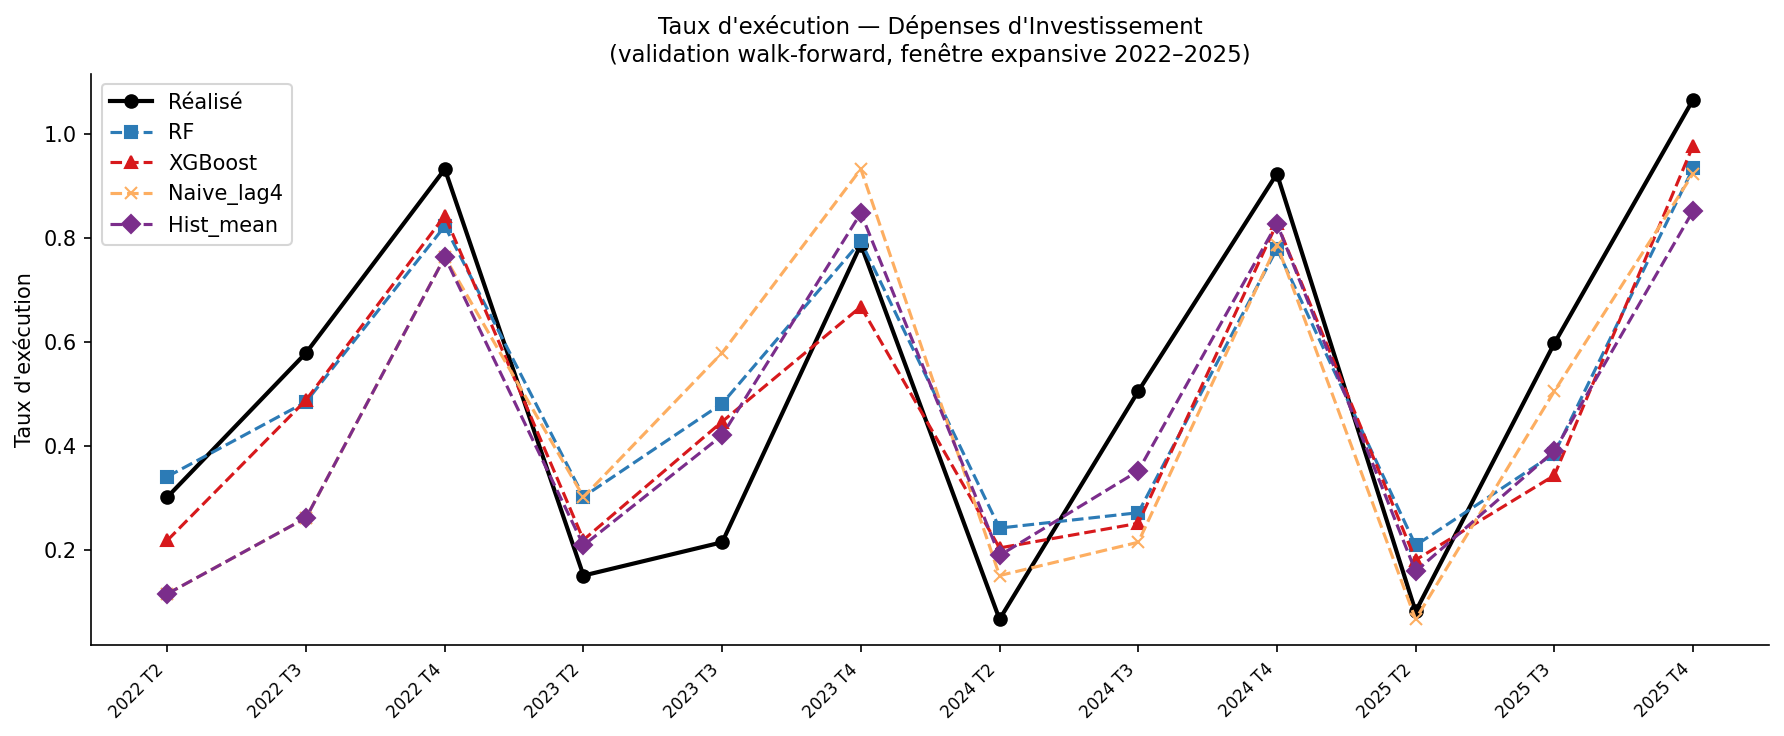
\includegraphics[width=0.85\textwidth]{figures/actual_vs_predicted_investissement.png}
    \caption{Taux d'ex\'ecution r\'eels vs pr\'evus par XGBoost --- cat\'egorie Investissement (folds 2022--2025).}
    \label{fig:actual-vs-pred}
\end{figure}

%================================================================
\phantomsection
\subsection*{4.6 \quad D\'etection d'anomalies}
\addcontentsline{toc}{subsection}{4.6 D\'etection d'anomalies}
%================================================================

Au-del\`a de la pr\'evision ponctuelle, le syst\`eme doit pouvoir signaler les
\textbf{comportements anormaux} qui appellent un examen approfondi.

%----------------------------------------------------------------
\phantomsection
\subsubsection*{4.6.1 \quad D\'efinition d'une anomalie d'ex\'ecution}
\addcontentsline{toc}{subsubsection}{4.6.1 D\'efinition d'une anomalie d'ex\'ecution}
%----------------------------------------------------------------

Une \textbf{anomalie d'ex\'ecution} est d\'efinie comme un comportement de la ligne
budg\'etaire \textit{statistiquement incompatible avec son propre historique}.
L'anomalie n'est pas une simple sous-ex\'ecution~: une ligne qui ex\'ecute syst\'ematiquement
\`a 60\,\% n'est pas anormale, m\^eme si son taux est faible. \`A l'inverse, une ligne
qui ex\'ecute habituellement \`a 95\,\% et tombe brutalement \`a 50\,\% \emph{est}
anormale, m\^eme si 50\,\% reste loin de z\'ero.

Cette d\'efinition relative est essentielle pour \'eviter deux \'ecueils~: les
faux positifs (lignes structurellement basses signal\'ees \`a tort) et les faux
n\'egatifs (anomalies r\'eelles masqu\'ees par un seuil absolu).

%----------------------------------------------------------------
\phantomsection
\subsubsection*{4.6.2 \quad M\'ethode : z-score sur l'historique T2 par ligne}
\addcontentsline{toc}{subsubsection}{4.6.2 M\'ethode : z-score sur l'historique T2 par ligne}
%----------------------------------------------------------------

Pour chaque ligne, on calcule la moyenne $\mu_i$ et l'\'ecart-type $\sigma_i$ des
taux T2 observ\'es sur les ann\'ees pass\'ees. Le \textbf{z-score} de l'observation
courante est~:
$$
z_i = \frac{\text{taux T2}_{2025} - \mu_i}{\sigma_i}
$$

\noindent
Une ligne est signal\'ee comme anormale si $z_i < -1{,}5$, c'est-\`a-dire si son
taux T2 actuel est inf\'erieur de plus de 1{,}5~\'ecart-type \`a sa moyenne historique.
La gradation suivante a \'et\'e adopt\'ee~:

\begin{itemize}
    \item \textbf{Mod\'er\'ee}~: $-2{,}0 \leq z < -1{,}5$.
    \item \textbf{S\'ev\`ere}~: $-3{,}0 \leq z < -2{,}0$.
    \item \textbf{Critique}~: $z < -3{,}0$ ou taux T2 nul.
\end{itemize}

\noindent
L'\'ecart-type est plafonn\'e \`a un minimum de 0{,}005 pour \'eviter qu'une ligne
\`a historique tr\`es stable ne d\'eclenche une alerte sur la moindre fluctuation.

%----------------------------------------------------------------
\phantomsection
\subsubsection*{4.6.3 \quad Anomalies identifi\'ees sur l'exercice 2025}
\addcontentsline{toc}{subsubsection}{4.6.3 Anomalies identifi\'ees sur l'exercice 2025}
%----------------------------------------------------------------

Sur les 130 lignes 2025, \textbf{4 anomalies} ont \'et\'e d\'etect\'ees
(tableau~\ref{tab:anomalies}).

\begin{table}[H]
\centering\small
\caption{Anomalies d'ex\'ecution d\'etect\'ees sur l'exercice 2025.}
\label{tab:anomalies}
\begin{tabular}{@{}p{6cm}p{4cm}c@{}}
\toprule
\textbf{Ligne budg\'etaire} & \textbf{R\'egion} & \textbf{Niveau} \\
\midrule
R\'ehabilitation des juridictions r\'egionales       & Guelmim-Oued Noun  & Mod\'er\'ee \\
Mat\'eriel m\'edical et sanitaire (prisons)          & Services communs   & Mod\'er\'ee \\
Fournitures \'etablissements p\'enitentiaires        & Services communs   & S\'ev\`ere   \\
Entretien et r\'eparation v\'ehicules - parc auto    & Services communs   & Mod\'er\'ee \\
\bottomrule
\end{tabular}
\end{table}

\noindent
Ces quatre signalements pointent tous vers des lignes op\'erationnelles \`a fort
impact (s\'ecurit\'e p\'enitentiaire, logistique, infrastructure judiciaire).
Le caract\`ere cibl\'e du signalement constitue pr\'ecis\'ement la valeur ajout\'ee
attendue d'un syst\`eme d'alerte pr\'ecoce~: focaliser l'attention des gestionnaires
sur quelques lignes critiques plut\^ot que de noyer le diagnostic dans la masse.

%================================================================
\phantomsection
\subsection*{4.7 \quad Synth\`ese, limites et conclusion}
\addcontentsline{toc}{subsection}{4.7 Synth\`ese, limites et conclusion}
%================================================================

Ce chapitre a pr\'esent\'e la cha\^ine compl\`ete de mod\'elisation~: construction et
description du jeu de donn\'ees, choix des variables, comparaison de quatre mod\`eles
selon un protocole sans fuite temporelle, s\'election d'une architecture sp\'ecialis\'ee
par cat\'egorie, et d\'etection statistique d'anomalies. Trois conclusions \'emergent~:

\begin{itemize}
    \item \textbf{Pr\'ecision diff\'erenci\'ee.} Le syst\`eme est tr\`es fiable sur le
    Personnel (RMSE 1{,}3~pp), bon sur le Mat\'eriel (6{,}8~pp), et utilisable
    \`a titre indicatif sur l'Investissement (14{,}6~pp).

    \item \textbf{Sp\'ecialisation gagnante.} Aucun mod\`ele unique n'est optimal sur
    toutes les cat\'egories~; combiner XGBoost, Lasso et moyenne historique selon
    le type de d\'epense am\'eliore la performance globale tout en restant transparent.

    \item \textbf{Anomalies cibl\'ees.} La d\'etection par z-score appliqu\'ee au
    taux T2 a identifi\'e quatre lignes pr\'esentant un comportement anormal pour
    l'exercice 2025, fournissant une base op\'erationnelle directement exploitable.
\end{itemize}

\textbf{Limites.} Trois limites doivent \^etre explicit\'ees. Premi\`erement, les taux
ligne par ligne sont \textbf{simul\'es} \`a partir d'agr\'egats publics~; les r\'esultats
constituent donc une preuve de concept, non une validation sur donn\'ees internes.
Deuxi\`emement, les \textbf{s\'eries sont courtes} (6 ann\'ees), ce qui limite la
capacit\'e des mod\`eles complexes \`a apprendre des relations fines et favorise
les approches parcimonieuses. Troisi\`emement, certaines \textbf{variables exog\`enes
potentiellement explicatives} (taux d'engagement, \'etat des march\'es publics,
disponibilit\'e des cr\'edits de paiement) ne sont pas int\'egr\'ees~; leur
exploitation, possible via une connexion au GID, constituerait l'\'etape suivante
naturelle de ce travail.

Le chapitre suivant pr\'esente la traduction de cette cha\^ine pr\'edictive en un
syst\`eme de pilotage op\'erationnel~: architecture logicielle, fonctionnalit\'es
du tableau de bord et apports attendus pour la Division de la Pr\'evision
et de la Programmation financi\`ere de la Direction du Budget.
